\documentclass{article}

% Language setting
% Replace `English' with e.g. `Spanish' to change the document language
\usepackage[english]{babel}
\usepackage[fontset=ubuntu]{ctex}

% Set page size and margins
% Replace `letter paper' with`a4paper' for UK/EU standard size
\usepackage[a4paper,top=1.5cm,bottom=1.5cm,left=2cm,right=2cm,marginparwidth=1.75cm]{geometry}

% Useful packages
\usepackage{float}
\usepackage{amsmath}
\usepackage{graphicx}
\usepackage{listings}
\usepackage{enumitem}
\usepackage[ruled]{algorithm2e}
\usepackage[colorlinks=true, allcolors=blue]{hyperref}

\SetKwProg{Function}{function}{:}{end}

\title{\heiti 计算机学院《算法设计与分析》第四次作业}
\author{114514 李田所}

\begin{document}
\maketitle

\section{判断正误并说明}

\begin{enumerate}[itemindent=3em]
    \item{存在一个$NP$完全问题可以在多项式时间内求解。}
    \item{若某$NP$问题不是多项式时间内可求解的,所有$NP$完全问题都不是多项式时间可求解的。}
    \item{判定无向图中是否存在环这一问题属于$P$问题。}
    \item{如果一个问题是$NP-hard$,则一定存在一个算法可以在多项式时间内验证该问题的解。}
\end{enumerate}

\subsection{命题一}

无法判断正误,目前还没有证明$P=NP$或$P\ne{NP}$。

\subsection{命题二}

正确,对任意$NP$完全问题,每一个$NP$问题都可以规约到它,因为存在一个不是多项式时间内可求解的$NP$问题到它的规约,此$NP$完全问题也不是多项式时间内可求解的。

\subsection{命题三}

正确,从任意一个节点开始进行$BFS$或$DFS$即可完成判断,时间复杂度为$O(V+E)$,显然是多项式时间复杂度,因此判定无向图中是否存在环这一问题属于$P$问题。

\subsection{命题四}

错误,考虑问题$\forall{x_1},\exists{x_2},f(x_1,x_2)=1$,其中$x_1,x_2$为$n$维的$0-1$向量。一方面存在$NP$完全问题$for\ a\ specified \ x_1,\exists{x_2},f(x_1,x_2)=1$到此问题的规约,从而这是一个$NP-hard$问题,另一方面由于$x_1$的任意性,不存在一个算法可以在多项式时间内验证该问题的解。从而可知如果一个问题是$NP-hard$,不一定存在一个算法可以在多项式时间内验证该问题的解。

\section{文件传送问题}

给定一个包含$n$个节点的图,图中包含$m$条单向边,起点和终点分别用$s_i$和$t_i$表示。现在需要选取一些节点为发送源,发送源会向外发送数据包,已知数据包只能沿图中单向边进行单向传播,且收到数据包的节点会将数据包通过以该节点为起点的单向边进行转发。

请设计一个高效算法计算最少需要几个发送源才能使所有节点收到数据包,写出该算法伪代码并分析时间复杂度。

\subsection{算法思想}

自然想到,对于每个入度为零的节点,都需要为其准备一个发射源,对于每个环,如果不存在可以到达这个环的数据包,则需要为环上任意一个节点准备一个发射源,因此可以循环寻找入度为零的节点进行处理直到全部节点被处理完毕。

具体的,如果找到了这样的节点就从这个节点开始搜索,被搜索到的全部节点都可以收到来自这个节点的数据包,因此可以删去这个节点和全部搜索到的节点,如果没有找到这样的节点,则表明此时的图由若干环组成,任意选择一个节点作为信号源开始搜索,同样删除这个节点和被搜索到的全部节点。

\begin{figure}[H]
\centering
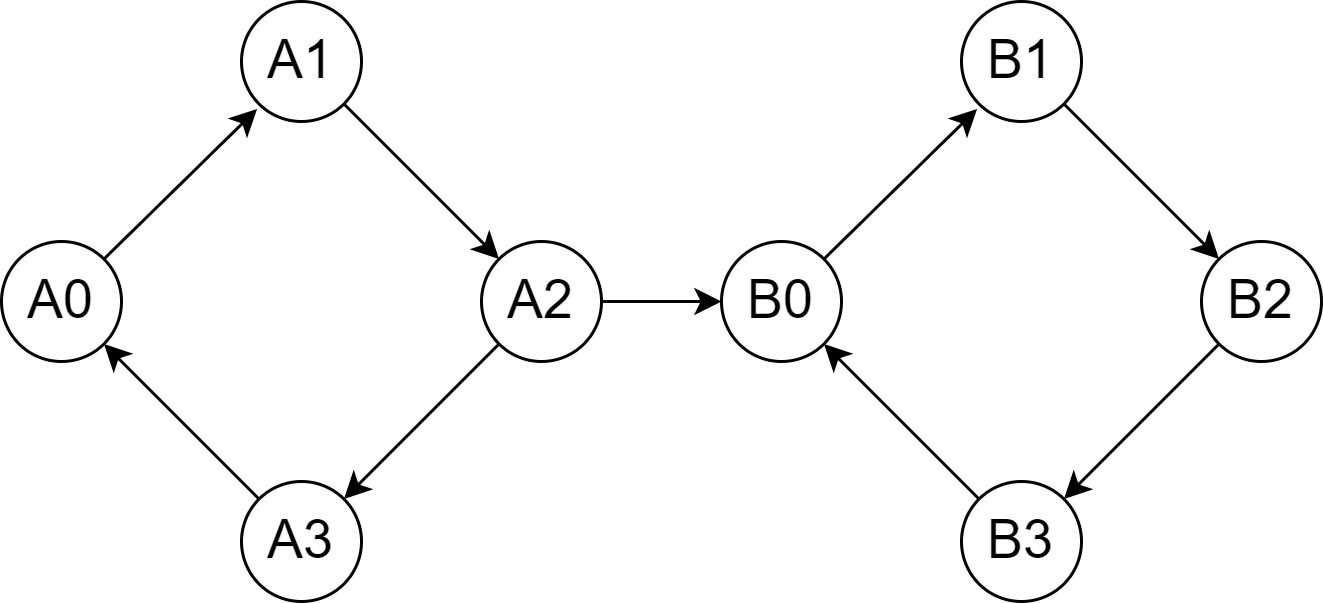
\includegraphics[width=0.3\textwidth]{algorithm_pic3.jpg}
\caption{文件传送问题}
\label{文件传送问题}
\end{figure}

简单思考即可发现,上述做法是存在问题的,对于环$A$和环$B$,若它们之间只被一条从$A$中某个节点到$B$中某个节点的单向边连接,且选择删除的节点在环$B$上,就会导致额外需要一个本不需要的发射源。注意到问题的关键在于环的影响,而环上任意一个节点可以收到数据包就意味着环上所有节点都可以收到数据包,可以将一个环视为一个节点处理,即通过求强连通分量进行缩点。

具体的,可使用$tarjan$算法求出强连通分量,将每一个强连通分量视为一个节点,从而得到一个新的有向无环图,这张有向无环图上入度为零的节点的个数即为所求,由于使用$tarjan$算法求出强连通分量的时间复杂度为$O(V+E)$,在缩点后的图上统计入度为零的节点的个数时间复杂度不超过$O(V+E)$,总时间复杂度为$O(V+E)$。

\subsection{伪代码与复杂度分析}

\begin{algorithm}[H]

\caption{文件传送问题}
\LinesNumbered
\KwIn{有向图G(V,E),包含$n$个节点$m$条边}
\KwOut{发送源数量的最小值$ans$}

\Function{$main(n,m,G)$}{
    $//\ setting\ global\ variables$\;
    $global\ input\ graph\ G$\;
    $global\ count\leftarrow0$\;
    $global\ colors\leftarrow0$\;
    $global\ stack\ for\ nodes$\;
    $global\ color\leftarrow[0,...,n-1]$\;
    $global\ low\leftarrow[0,...,n-1]\ with\ 0\ inited$\;
    $global\ dfn\leftarrow[0,...,n-1]\ with\ 0\ inited$\;
    $global\ vis\leftarrow[0,...,n-1]\ with\ false\ inited$\;
    \For{$i\leftarrow0\ to\ n-1$}{
        \If{$dfn[i]=0$}{
            $call\ tarjan(i)$\;
        }
    }
    $ans\leftarrow{call}\ check()$\;
    \textbf{$return\ ans$}\;
}

\end{algorithm}

此算法需要使用较多的全局数据结构,出于简洁考虑,全部全局定义在$main$函数中给出,并使用$global$进行标记以便区分。

在$main$函数中,循环调用了$tarjan$函数求解强连通分量,调用的条件为$dfn[i]=0$,注意到对于每一个$i$,在$main$函数或$tarjan$函数中,$dfn[i]$只会被更新一次成为非零值,可知$tarjan$函数的执行次数为$n$(包括递归调用),全部对$tarjan$函数的调用总计是$O(n+m)$复杂度的(具体见接下来$tarjan$部分的分析),而调用$check$的函数也是$O(n+m)$复杂度的(具体见接下来$check$部分的分析),从而此做法的总时间复杂度为$O(n+m)$,其中$n$表示图中点数,$m$表示图中边数。

\begin{algorithm}[H]

\caption{文件传送问题}
\LinesNumbered
\KwIn{有向图G(V,E),包含$n$个节点$m$条边}
\KwOut{发送源数量的最小值$ans$}

\Function{$tarjan(src)$}{
    $//\ using\ global\ variables$\;
    $count\leftarrow{count}+1$\;
    $vis[src]\leftarrow{true}$\;
    $dfn[src]\leftarrow{count}$\;
    $low[src]\leftarrow{count}$\;
    $push\ src\ in\ stack$\;
    \For{$i\in{Adj}(src)$}{
        \If{$dfn[i]=0$}{
            $call\ tarjan(i)$\;
            $low[src]\leftarrow{min}(low[src],low[i])$\;
        }
        \ElseIf{$vis[i]$}{
            $low[src]\leftarrow{min}(low[src],dfn[i])$\;
        }
    }
    \If{$dfn[src]=low[src]$}{
        $vis[src]\leftarrow{false}$\;
        $color[src]\leftarrow{colors}$\;
        \While{$stack\ is\ not\ empty\ and\ stack.top\ne{src}$}{
            $vis[stack.top]\leftarrow{false}$\;
            $color[stack.top]\leftarrow{colors}$\;
            $pop\ stack$\;
        }
        $colors\leftarrow{colors}+1$\;
        $pop\ stack$\;
    }
}

\end{algorithm}

对于图中每一个节点$i$,$dfn[i]$只会被更新一次成为非零值,即这个节点只会被访问一次,因此第$8-16$行的循环在全部对$tarjan$函数的调用中,访问了图中全部的边,是$O(m)$复杂度的,第$17-27$行为着色过程,每个节点会被且仅会被着色一次,在全部对$tarjan$函数的调用中,着色了图中全部的节点,是$O(n)$复杂度的,因此全部对$tarjan$函数的调用总计是$O(n+m)$复杂度的,其中$n$表示图中点数,$m$表示图中边数。

\begin{algorithm}[H]

\caption{文件传送问题}
\LinesNumbered
\KwIn{有向图G(V,E),包含$n$个节点$m$条边}
\KwOut{发送源数量的最小值$ans$}

\Function{$check(src)$}{
    $//\ using\ global\ variables$\;
    $check\leftarrow[0,...,colors-1]\ with\ 0\ inited$\;
    \For{$i\leftarrow0\ to\ n-1$}{
        \For{$j\in{Adj}(i)$}{
            \If{$color[i]\ne{color}[j]$}{
                $check[color[j]]\leftarrow{check}[color[j]]+1$\;
            }
        }
    }
    $ans\leftarrow0$\;
    \For{$i\leftarrow0\ to\ colors-1$}{
        \If{$check[i]=0$}{
            $ans\leftarrow{ans}+1$\;
        }
    }
    \textbf{$return\ ans$}\;
}

\end{algorithm}

$4-10$行的二层循环遍历了图中全部的节点和全部的边,显然是$O(n+m)$复杂度的,而$12-16$行的循环执行次数为$colors$,最坏情况下图中的节点两两不连通,此时$colors=n$,否则$colors<n$,因此这一部分的时间复杂度不超过$O(n)$,总时间复杂度为$O(n+m)$,其中$n$表示图中点数,$m$表示图中边数。

\section{最小环问题}

给定一个包含$n$个点的无向图,边权使用矩阵$w_{i,j}(w_{i,j}>0)$表示。

请设计一个高效的算法,计算图中最小环(最少包含三个节点)的最小边权和,写出该算法伪代码并分析时间复杂度。

\begin{figure}[H]
\centering
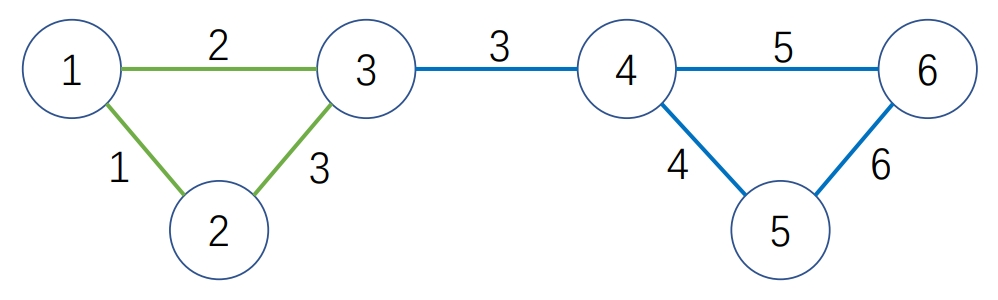
\includegraphics[width=0.5\textwidth]{algorithm_pic1.jpg}
\caption{无向图最小环}
\label{无向图最小环}
\end{figure}

如图\ref{无向图最小环}所示,节点$1-2-3$组成的环权重为$6$,是该图中的最小环,节点$4-5-6$组成的环权重为$15$,不能被称为该图中的最小环,节点$3-4$不满足最少包含三个节点的条件,不能被称为该图中的最小环。

\subsection{算法思想}

对于以邻接矩阵形式输入的图,自然想到用$Floyd$算法计算多源最短路,$Floyd$算法本质上是空间优化后的动态规划,因此对于最小环问题的求解也可以类比$Floyd$算法,使用空间优化后的动态规划。

以$k$表示前$k$个节点的集合,$Floyd$算法的状态转移方程如下:

$$
dp_{ij}^k=min(dp_{ij}^{k-1},dp_{ik}^{k-1}+dp_{kj}^{k-1})
$$

在此基础上,考虑增加第$k$个节点的时候,最小环变化的情况,对于每个$k$,新增的环路为:

$$
shortest\_path_{ij}+weight_{ki}+weight_{kj}
$$

其中$shortest\_path_{ij}$表示只使用前$k-1$个节点的$i$到$j$的最短路径,可以在$Floyd$算法每一轮状态转移开始之前直接获得,即在枚举$i$和$j$更新$dp$之前,先枚举$i$和$j$更新最小环:

$$
min\_cycle=min(min\_cycle,shortest\_path_{ij}+weight_{ki}+weight_{kj})
$$

需要注意的是,枚举环路时的$i$和$j$需要满足$i\ne{j},i<k,j<k$,对于无向图可进一步简化为$i<j<k$,由于包含了三层$O(V)$的循环,此做法总时间复杂度为$O(V^3)$。

\subsection{伪代码与复杂度分析}

\begin{algorithm}[H]

\caption{最小环问题}
\LinesNumbered
\KwIn{矩阵$w$,矩阵的长和宽均为$n$}
\KwOut{最小环(最少包含三个节点)的最小边权和$ans$}

\Function{$main(n,w[])$}{
    $dis\leftarrow{w}$\;
    $ans\leftarrow+\infty$\;
    \For{$k\leftarrow0\ to\ n-1$}{
        \For{$i\leftarrow0\ to\ n-1$}{
            \For{$j\leftarrow0\ to\ n-1$}{
                \If{$i<j<k$}{
                    $ans\leftarrow{min}(ans,dis[i][j]+w[i][k]+w[j][k])$\;
                }
                $dis[i][j]\leftarrow{min}(dis[i][j],dis[i][k]+dis[k][j])$\;
            }
        }
    }
    \textbf{$return\ ans$}\;
}

\end{algorithm}

显然$4-13$行的循环执行了$n$次,$5-12$行的循环执行了$n$次,$6-11$行的循环执行了$n$次,$7-10$行的复杂度是$O(1)$。因此$6-11$行的循环复杂度为$O(n)$,$5-12$行的循环复杂度为$O(n^2)$,$4-13$行的循环复杂度为$O(n^3)$,从而此做法的总时间复杂度为$O(n^3)$。

\section{哈密顿路径问题}

哈密顿路径$(Hamiltonian\ path)$是指图中每个节点都仅经过一次且必须经过一次的路径。对于一般的图结构来说,求解哈密顿路径的问题是$NP$难问题。然而,在有向无环图上寻找哈密顿路径的问题是存在多项式时间的解法的。

\begin{figure}[H]
\centering
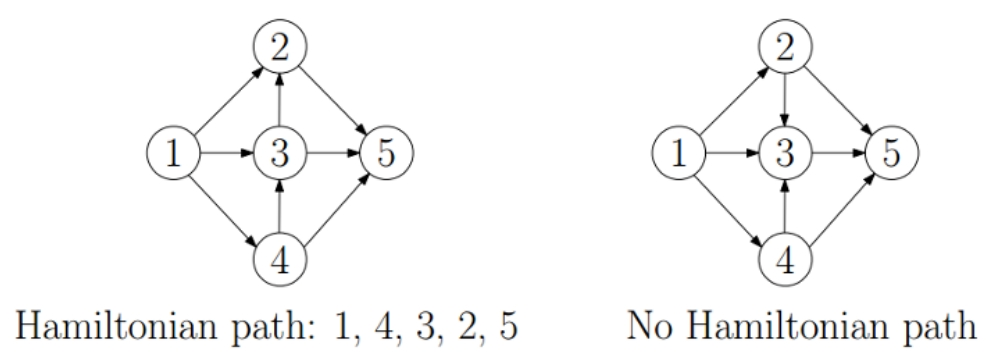
\includegraphics[width=0.6\textwidth]{algorithm_pic2.jpg}
\caption{哈密顿路径}
\label{哈密顿路径}
\end{figure}

如图\ref{哈密顿路径}所示,左侧图包含一条哈密顿路径$1-4-3-2-5$,右侧图则不包含哈密顿路径。

给定一个有向无环图$G=(V,E)$,请设计一个高效算法来寻找图$G$的一条哈密顿路径,如不存在哈密顿路径则返回$−1$,写出该算法伪代码并分析时间复杂度。

\subsection{算法思想}

由于处理的图具有有向无环的性质,自然想到类似拓扑排序进行处理,每次选择一个入度为零的节点并删去这个节点,直到删除全部的$n$个节点算法结束。在处理哈密顿路径问题时,需要对上述过程进行一些处理,在不存在哈密顿路径时结束算法:

\begin{itemize}[itemindent=3em]
    \item{在任意时刻(初始化时,删除节点后更新时)如果同时存在不止一个入度为$0$的节点,则不存在一条经过图中每一个节点的路径,因此也不存在哈密顿路径。}
    \item{算法结束时,被访问的节点数量不到$n$,说明图中可能存在环,对于一个有向无环图无需处理这种情况,可以返回不存在哈密顿路径。}
\end{itemize}

\begin{figure}[H]
\centering
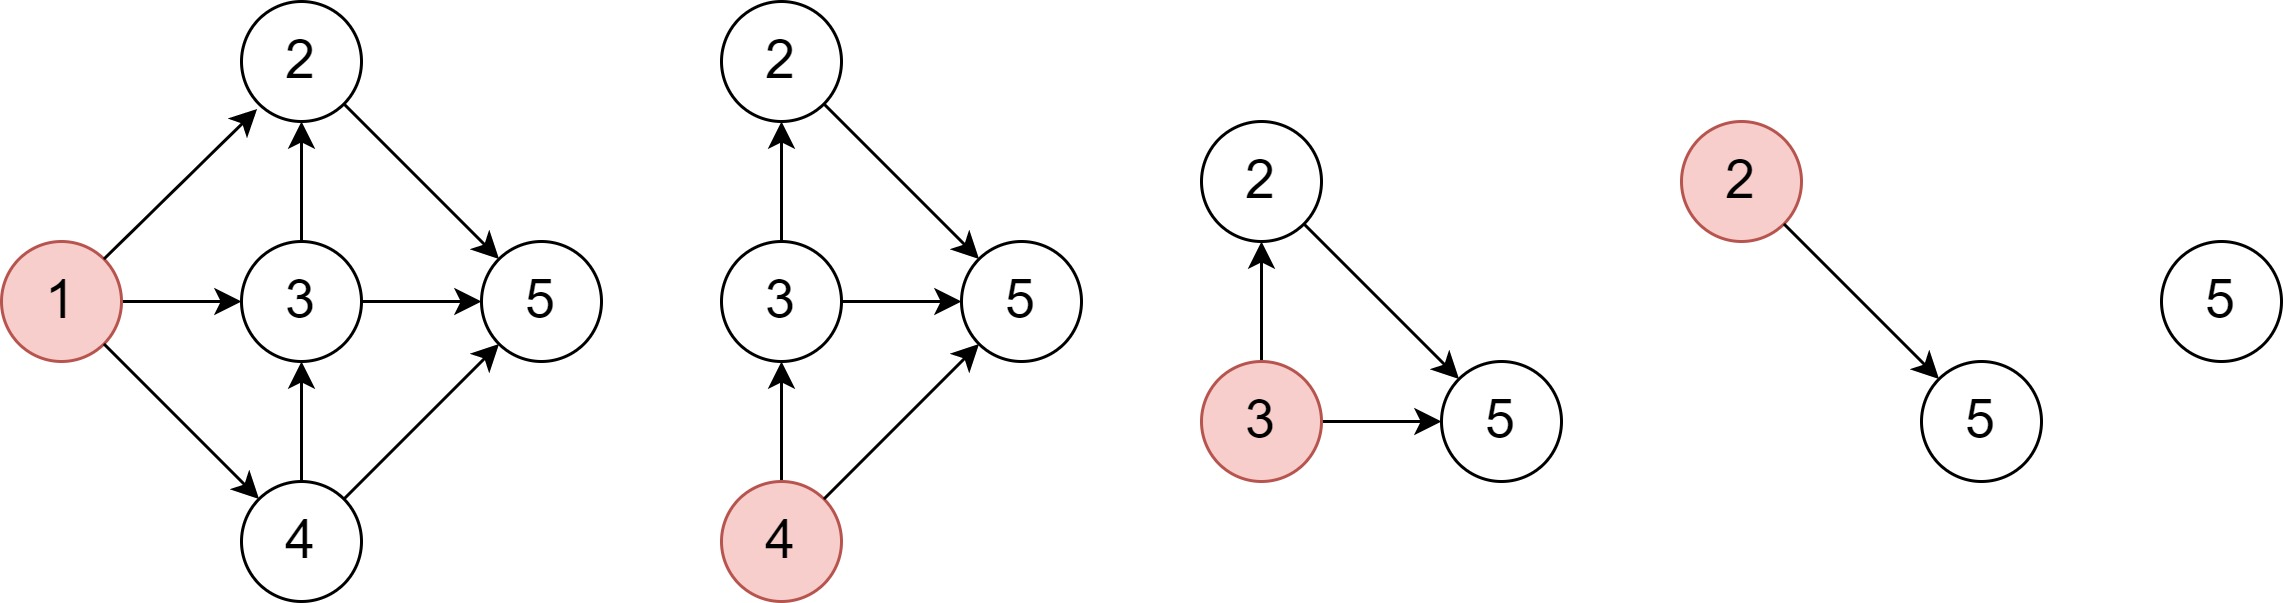
\includegraphics[width=0.7\textwidth]{algorithm_pic4.jpg}
\caption{存在哈密顿路径}
\label{存在哈密顿路径}
\end{figure}

\begin{figure}[H]
\centering
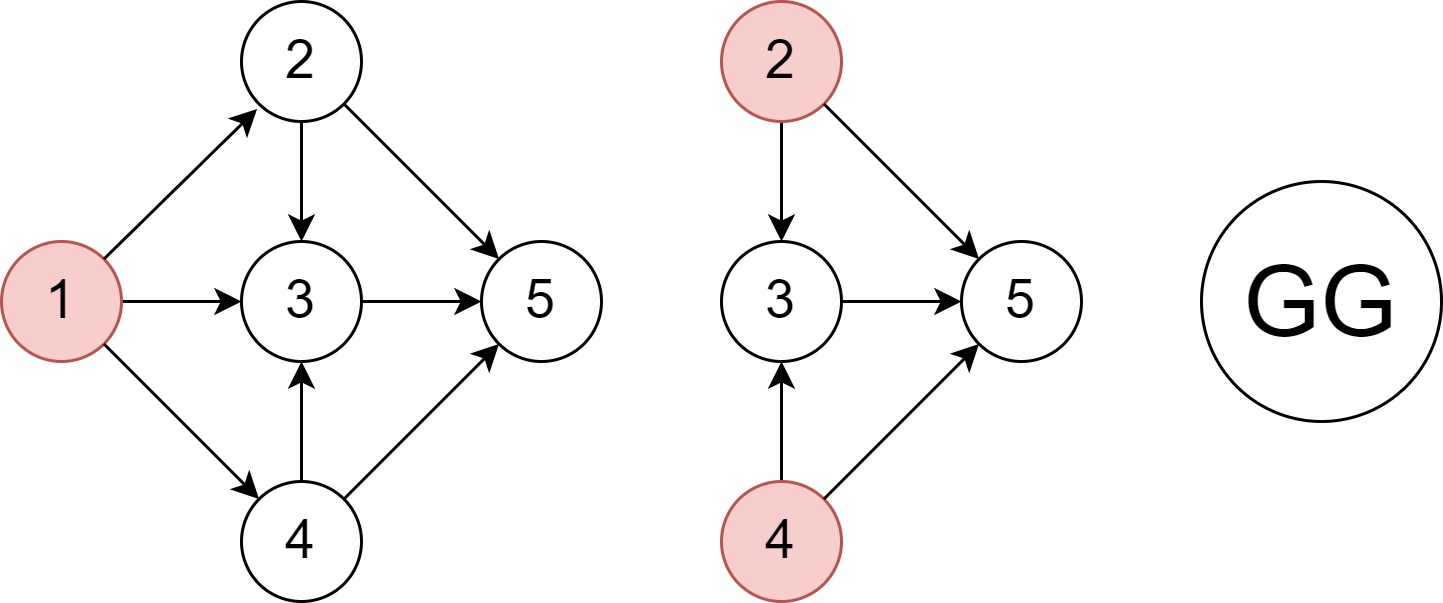
\includegraphics[width=0.45\textwidth]{algorithm_pic5.jpg}
\caption{不存在哈密顿路径}
\label{不存在哈密顿路径}
\end{figure}

在进行拓扑排序时,我们使用了一个队列维护入度为零的节点的集合,在此问题中,由于存在不止一个入度为零的节点时算法直接退出,我们可以简单的使用一个变量表示入度为零的节点,由于在存在哈密顿路径(没有提前返回不存在哈密顿路径)的情况下,我们访问了每个节点一次,且对于每个节点访问其全部的出边一次,总时间复杂度为$O(V+E)$。

\subsection{伪代码与复杂度分析}

\begin{algorithm}[H]

\caption{哈密顿路径问题}
\LinesNumbered
\KwIn{有向图G(V,E),包含$n$个节点$m$条边}
\KwOut{数组$ans$,为一条哈密顿路径,或$-1$,表示不存在哈密顿路径}

\Function{$main(n,m,G)$}{
    $count\leftarrow[0,...,n-1]$\;
    \For{$i\leftarrow0\ to\ n-1$}{
        $count[i]\leftarrow{in\_degree}[i]$\;
    }
    $start\leftarrow-1$\;
    \For{$i\leftarrow0\ to\ n-1$}{
        \If{$count[i]=0$}{
            \If{$start\ne-1$}{
                \textbf{$return\ -1$}\;
            }
            $start\leftarrow{i}$\;
        }
    }
    $index\leftarrow0$\;
    $order\leftarrow[0,...,n-1]$\;
    \While{$start\ne-1$}{
        $order[index]\leftarrow{start}$\;
        $index\leftarrow{index}+1$\;
        $temp\leftarrow{start}$\;
        $start\leftarrow-1$\;
        \For{$i\in{Adj}(temp)$}{
            $count[i]\leftarrow{count}[i]-1$\;
            \If{$count[i]=0$}{
                \If{$start\ne-1$}{
                    \textbf{$return\ -1$}\;
                }
                $start\leftarrow{i}$\;
            }
        }
    }
    \If{$index\ne{n}$}{
        \textbf{$return\ -1$}\;
    }
    \textbf{$return\ ans$}\;
}

\end{algorithm}

对于$3-5$和$7-14$行的循环,循环的执行次数至多为$n$,时间复杂度为$O(n)$,对于$17-31$行的循环,在不提前返回的情况下,每一轮循环将$index$增加了$1$,$index$至多增加到$n$,时间复杂度为$O(n)$,而$22-30$行的循环访问了当前节点的全部出边,在全部的$17-31$行的循环中,访问了图中全部的边,是$O(m)$复杂度的,从而此做法的总时间复杂度为$O(n+m)$,其中$n$表示图中点数,$m$表示图中边数。

\section{二分图判定问题}

二分图是指一个无向图$G=(V,E)$,它的所有顶点可被分成两个子集,且同一个子集中任何两顶点间都没有边相连。(换言之,$G$为二分图,当且仅当存在两个集合$V_1,V_2$满足$V_1\cup{V_2}=V,V_1\cap{V_2}=\emptyset$,$E$中每条边都连接了$V_1$中某个点与$V_2$中某个点。)

\begin{enumerate}[itemindent=3em]
    \item{请证明:二分图中不存在长度为奇数的环。}
    \item{请设计一个基于广度优先搜索$(BFS)$的算法来判断无向图$G$是否为二分图,写出该算法伪代码并分析该算法时间复杂度。}
\end{enumerate}

\subsection{证明二分图中不存在长度为奇数的环}

假设二分图$G=(V,E)$中存在一个长为$2n+1$的环,环上的节点依次是$<a_0,a_1,...,a_{2n}>$,集合$V_1,V_2$满足$V_1\cup{V_2}=V,V_1\cap{V_2}=\emptyset$,$E$中每条边都连接了$V_1$中某个节点与$V_2$中某个节点。

不妨设$a_0\in{V_1}$由于$a_i,a_{i+1}$之间存在一条边,而$E$中每条边都连接了$V_1$中某个节点与$V_2$中某个节点,可知$a_i$和$a_{i+1}$不同在$V_1$或$V_2$,从而$a_1\in{V_2},a_2\in{V_1},...,a_{2n}\in{V_1}$,由于$a_{2n},a_0$之间存在一条边,可知存在一条起点和终点都在$V_1$或$V_2$中的边,这与$G=(V,E)$是二分图矛盾。

\begin{figure}[H]
\centering
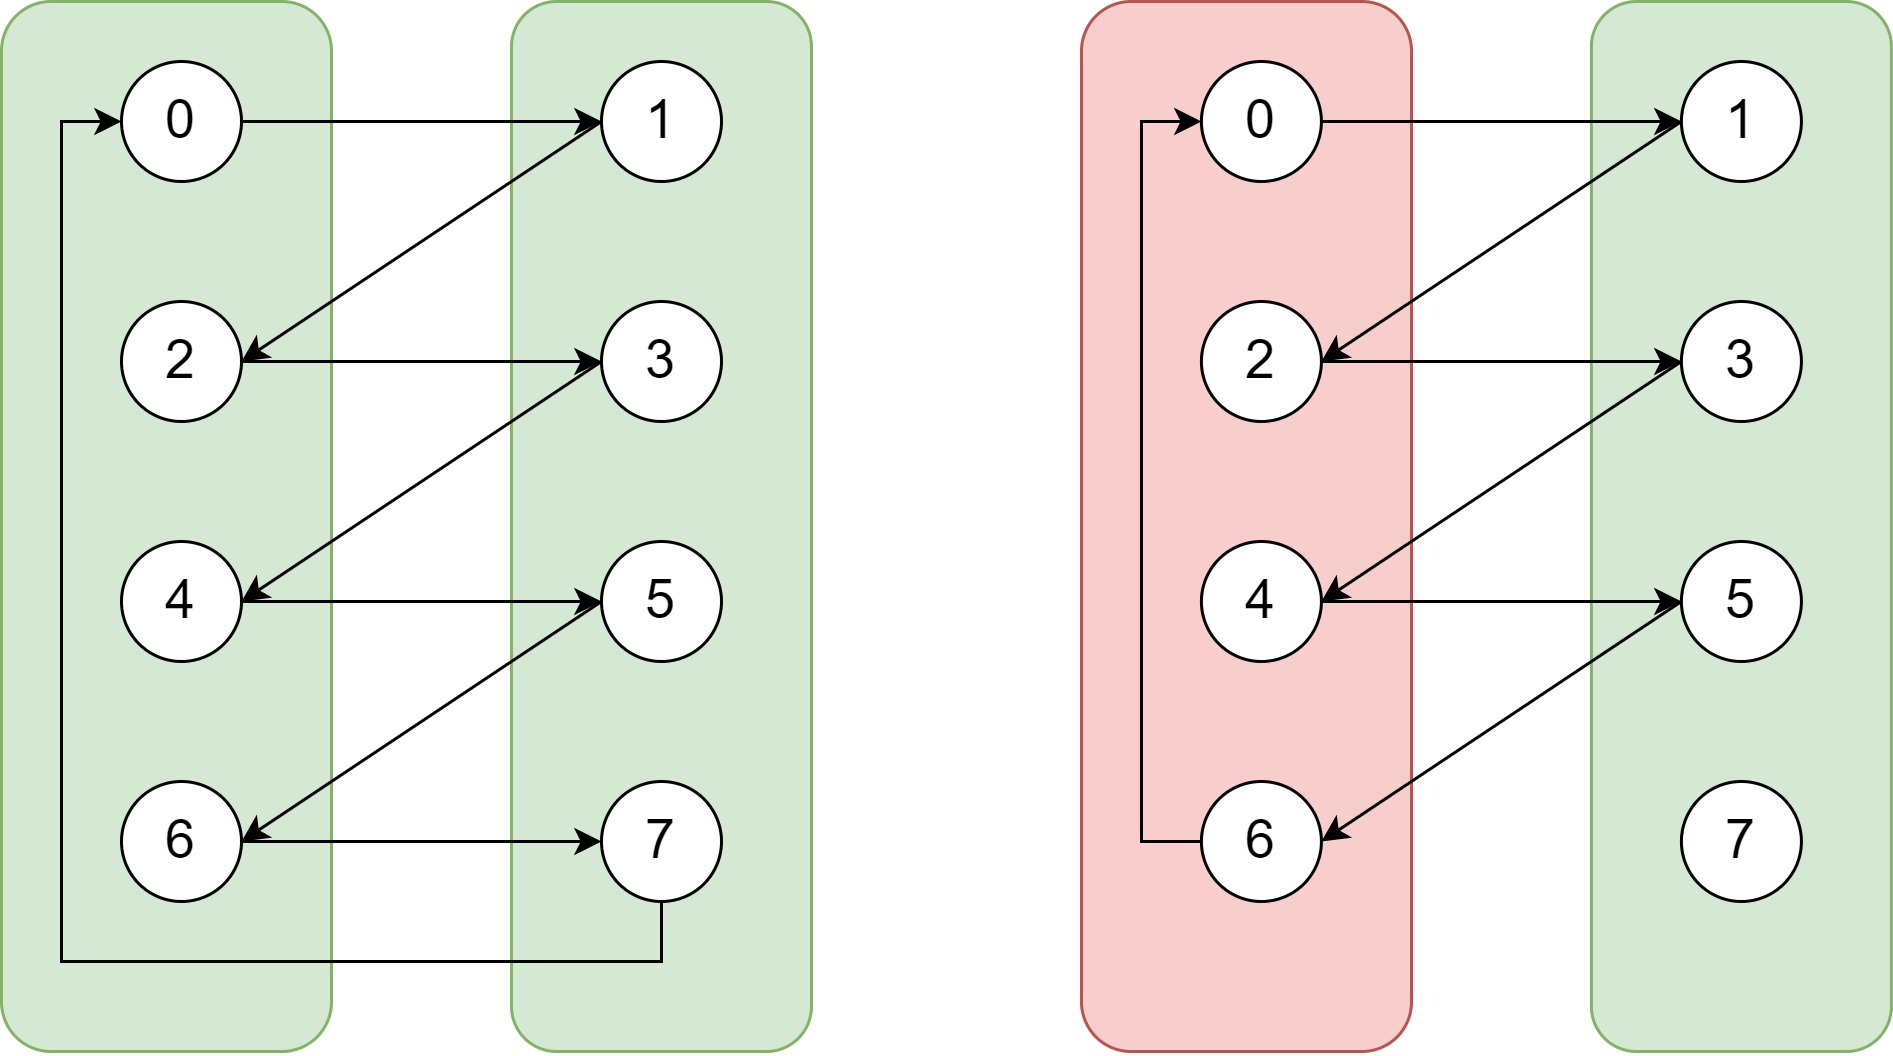
\includegraphics[width=0.7\textwidth]{algorithm_pic6.jpg}
\caption{二分图判定问题}
\label{二分图判定问题}
\end{figure}

由上可知,假设不成立,二分图中不存在长度为奇数的环。

\subsection{算法思想}

容易想到使用$BFS$计算图中各个节点到任取的源点的距离,如果某个节点$A$连接的节点$B$到源点距离已经被计算,记节点$A$到源点的距离为$dis_A$,节点$B$到源点的距离为$dis_B$,连接$AB$将形成长度为$dis_A+dis_B+1$的环,由上述结论“二分图中不存在长度为奇数的环”可知,$dis_A+dis_B+1$为偶数,$dis_A+dis_B$为奇数,即$dis_A$和$dis_B$不同奇偶。

因此只要在$BFS$的基础上,入队时额外进行检查,对于到源点距离已经被计算的节点,验证其与当前访问的节点的奇偶性是否一致即可,由于本质仍是图上$BFS$,显然时间复杂度为$O(V+E)$。

\subsection{伪代码与复杂度分析}

\begin{algorithm}[H]

\caption{二分图判定问题}
\LinesNumbered
\KwIn{无向图G(V,E),包含$n$个节点$m$条边}
\KwOut{布尔值$ans$,$ans$为真表示图$G$是完全图,否则$G$不是完全图}

\Function{$main(n,m,G)$}{
    $queue\ for\ nodes$\;
    $dis\leftarrow[0,...,n-1]\ with\ -1\ inited$\;
    \For{$i\leftarrow0\ to\ n-1$}{
        \If{$dis[i]<0$}{
            $dis[i]\leftarrow0$\;
            $push\ i\ in\ queue$\;
            \While{$queue\ is\ not\ empty$}{
                $top\leftarrow{queue}.head$\;
                $pop\ queue$\;
                \For{$j\in{Adj}(top)$}{
                    \If{$dis[i]<0$}{
                        $dis[j]\leftarrow{dis}[top]+1$\;
                        $push\ j\ in\ queue$\;
                    }
                    \ElseIf{$dis[j]\equiv{dis}[top]\ (mod\ 2)$}{
                        \textbf{$return\ false$}\;
                    }
                }
            }
        }
    }
    \textbf{$return\ true$}\;
}

\end{algorithm}

上述过程是一个可能因$return\ false$提前结束的图上$BFS$的过程,$4-22$行的外层循环和$6-20$行的广度优先搜索中,图上$n$个节点每个节点被访问了一次,访问后不会再满足$dis[i]<0$,不会被再次访问,是$O(n)$复杂度的,$11-19$行的循环中遍历了当前访问的节点的全部出边,结合上面的分析可知,全部节点的全部出边被访问了一次,是$O(m)$复杂度的,从而此做法的总时间复杂度为$O(n+m)$,其中$n$表示图中点数,$m$表示图中边数。

\section{附录暨部分算法的实现}

\subsection{文件传送问题C++实现}

\definecolor{mygreen}{rgb}{0,0.6,0}
\definecolor{mygray}{rgb}{0.5,0.5,0.5}
\definecolor{mymauve}{rgb}{0.58,0,0.82}

\lstset{
    backgroundcolor=\color{white},   % choose the background color; you must add \usepackage{color} or \usepackage{xcolor}
    basicstyle=\footnotesize,        % the size of the fonts that are used for the code
    breakatwhitespace=false,         % sets if automatic breaks should only happen at whitespace
    breaklines=true,                 % sets automatic line breaking
    captionpos=bl,                   % sets the caption-position to bottom
    commentstyle=\color{mygreen},    % comment style
    deletekeywords={...},            % if you want to delete keywords from the given language
    escapeinside={\%*}{*)},          % if you want to add LaTeX within your code
    extendedchars=true,              % lets you use non-ASCII characters; for 8-bits encodings only, does not work with UTF-8
    frame=single,                    % adds a frame around the code
    keepspaces=true,                 % keeps spaces in text, useful for keeping indentation of code (possibly needs columns=flexible)
    keywordstyle=\color{blue},       % keyword style
    language=c++,                    % the language of the code
    morekeywords={*,...},            % if you want to add more keywords to the set
    numbers=left,                    % where to put the line-numbers; possible values are (none, left, right)
    numbersep=5pt,                   % how far the line-numbers are from the code
    numberstyle=\tiny\color{mygray}, % the style that is used for the line-numbers
    rulecolor=\color{black},         % if not set, the frame-color may be changed on line-breaks within not-black text (e.g. comments (green here))
    showspaces=false,                % show spaces everywhere adding particular underscores; it overrides 'showstringspaces'
    showstringspaces=false,          % underline spaces within strings only
    showtabs=false,                  % show tabs within strings adding particular underscores
    stepnumber=1,                    % the step between two line-numbers. If it's 1, each line will be numbered
    stringstyle=\color{mymauve},     % string literal style
    tabsize=2,                       % sets default tabsize to 2 spaces
}

\begin{lstlisting}
#include <stack>
#include <cstdio>
#include <vector>
using namespace std;

int n,m,count,colors;
vector<vector<int>> graph;

stack<int> stk;
vector<bool> vis;
vector<int> dfn,low,color;

void tarjan(int src)
{
	dfn[src]=low[src]=++count;
	vis[src]=true,stk.push(src);
	for (int i : graph[src])
	{
		if (!dfn[i]) tarjan(i),low[src]=min(low[src],low[i]);
		else if (vis[i]) low[src]=min(low[src],dfn[i]);
	}
	if (dfn[src]==low[src])
	{
		vis[src]=false,color[src]=colors;
		while (!stk.empty() && stk.top()!=src)
		{
			color[stk.top()]=colors;
			vis[stk.top()]=false;
			stk.pop();
		}
		colors++,stk.pop();
	}
}

int main()
{
	int ans=0;
	scanf("%d %d",&n,&m);
	graph.resize(n),vis.resize(n,false);
	dfn.resize(n,0),low.resize(n,0),color.resize(n,0);
	for (int s,t,i=0;i<m;i++)
	{
		scanf("%d %d",&s,&t);
		graph[s].push_back(t);
	}
	for (int i=0;i<n;i++) if (!dfn[i]) tarjan(i);
	vector<int> check(colors,0);
	for (int i=0;i<n;i++) for (int j : graph[i])
		if (color[i]-color[j]) check[color[j]]++;
	for (int i : check) if (!i) ans++;
	printf("%d\n",ans);
	return 0;
}
\end{lstlisting}

\subsection{最小环问题C++实现}

\begin{lstlisting}
#include <cstdio>
#include <vector>
using namespace std;

const int inf=100000000;

int main()
{
	int n,ans=inf; scanf("%d",&n);
	vector<vector<int>> dis(n,vector<int>(n,0));
	vector<vector<int>> graph(n,vector<int>(n,0));
	for (int i=0;i<n;i++) for (int j=0;j<n;j++) scanf("%d",&graph[i][j]);
	for (int i=0;i<n;i++) for (int j=0;j<n;j++) dis[i][j]=graph[i][j];
	for (int k=0;k<n;k++) for (int i=0;i<n;i++) for (int j=0;j<n;j++)
	{
		if (i<j && j<k) ans=min(ans,dis[i][j]+graph[i][k]+graph[j][k]);
		dis[i][j]=min(dis[i][j],dis[i][k]+dis[k][j]);
	}
	if (ans<inf) printf("%d\n",ans);
	else puts("nan");
	return 0;
}
\end{lstlisting}

\subsection{哈密顿路径问题C++实现}

\begin{lstlisting}
#include <vector>
#include <cstdio>
using namespace std;

int main()
{
	int n,m;
	scanf("%d %d",&n,&m);
	vector<int> count(n);
	vector<vector<int>> ins(n);
	vector<vector<int>> outs(n);
	for (int s,t,i=0;i<m;i++)
	{
		scanf("%d %d",&s,&t);
		outs[s].push_back(t);
		ins[t].push_back(s);
	}
	int start=-1;
	for (int i=0;i<n;i++)
	{
		count[i]=ins[i].size(); if (count[i]==0)
		{
			if (start==-1) start=i;
			else {printf("%d\n",-1); return 0;}
		}
	}
	vector<int> order;
	while (start!=-1)
	{
		order.push_back(start),start=-1;
		for (int i : outs[order[order.size()-1]])
		{
			count[i]--; if (count[i]==0)
			{
				if (start==-1) start=i;
				else {printf("%d\n",-1); return 0;}
			}
		}
	}
	if ((int)order.size()==n) for (int i : order) printf("%d ",i);
	else printf("%d",-1); puts("");
	return 0;
}
\end{lstlisting}

\subsection{二分图判定问题C++实现}

\begin{lstlisting}
#include <queue>
#include <cstdio>
#include <vector>
using namespace std;

int main()
{
	int n,m; scanf("%d %d",&n,&m);
	vector<int> dis(n,-1);
	vector<vector<int>> graph(n);
	for (int s,t,i=0;i<m;i++)
	{
		scanf("%d %d",&s,&t);
		graph[s].push_back(t);
		graph[t].push_back(s);
	}
	queue<int> que;
	for (int i=0;i<n;i++) if (dis[i]<0)
	{
		dis[i]=0,que.push(i);
		while (!que.empty())
		{
			int top=que.front(); que.pop();
			for (int j : graph[top])
			{
				if (dis[j]<0) dis[j]=dis[top]+1,que.push(j);
				else if ((~dis[j]^dis[top])&1) {puts("false"); return 0;}
			}
		}
	}
	puts("true");
	return 0;
}
\end{lstlisting}

\subsection{随机图生成C++实现}

\begin{lstlisting}
#include <set>
#include <cstdio>
#include <random>
#include <utility>
using namespace std;

mt19937 generator(0x19260817);

int main()
{
	int n=15000,m=60000;
	printf("%d %d\n",n,m);
	set<pair<int,int>> unique;
	for (int i=0;i<m;i++)
	{
		int x=generator()%n;
		int y=generator()%n;
		pair<int,int> gen(x,y);
		if (unique.find(gen)!=unique.end()) {i--; continue;}
		printf("%d %d\n",x,y);
	}
	return 0;
}
\end{lstlisting}

\end{document}